\chapter{Referencial Teórico}\label{cap:referencial_teorico}

\section{Twitter}\label{sec:twitter}

* Como começou
* Objetivo (visão) do Twitter
* Princípios 140 caracteres, hashtags
* Quantidade de usuários ativos, alcance, volume de informações
* Relevância para estudos estatísticos de natureza comportamental

O Twitter é conhecido como um \emph{microblog} fundado em março de 2006 por Jack Dorsey, Evan Williams e Biz Stone. Ele consiste em pequenas publicações de até 140 caracteres, conhecidas como \emph{tweet}, que tem como objetivo possibilitar que o usuário se expresse de forma rápida e resumida. No corpo de um \emph{tweet}, o usuário pode fazer uso de marcadores conhecidos como \emph{hashtags} \cite{waite2012paperback}, para vincular aquela mensagem à um tópico específico. Com o uso massivo de marcadores em palavras ou frases gera uma grande massa de \emph{tweets} foi criado os \emph{trending topics}, em tradução livre seria os "assuntos mais comentados" onde é mostrado o qual relevante aquele marcador está em determinado lugar, de escolha do usuário, como: Brasil, Mundo, Rio de Janeiro ou outra qualquer localidade. O twitter de acordo com  faz uso de \emph{machine learning} para identificar e classificar o idioma da mensagem escrita pelo usuário \cite{arneromannkurrik2013}.


\section{Mineração de opinião}\label{sec:mineracao_dados}

* O que é?* Exemplos no mercado* Etapas(http://www.inf.ufsc.br/~alvares/INE5644/MineracaoOpiniao.pdf)

É de conhecimento comum que há um acúmulo de dados por toda a internet. Artigos, informações de usuários, comportamento de usuários, essas são alguns tipos de informação que pode ser encontrada hoje na internet. Esse grande acumulo não garante informações confiáveis ou uma análise correta sobre os dados, por isso hoje há uma grande urgência para novas teorias computacionais e ferramentas que ajudem a analisar essa quantidade de dados que só aumenta \cite{fayyad1996data}. E dentro dessa enorme gama de dados, existem as informações adicionadas por usuários através de texto que remetem a suas reações a determinadas situações ou objetos.


\begin{figure}[ht]
	\centering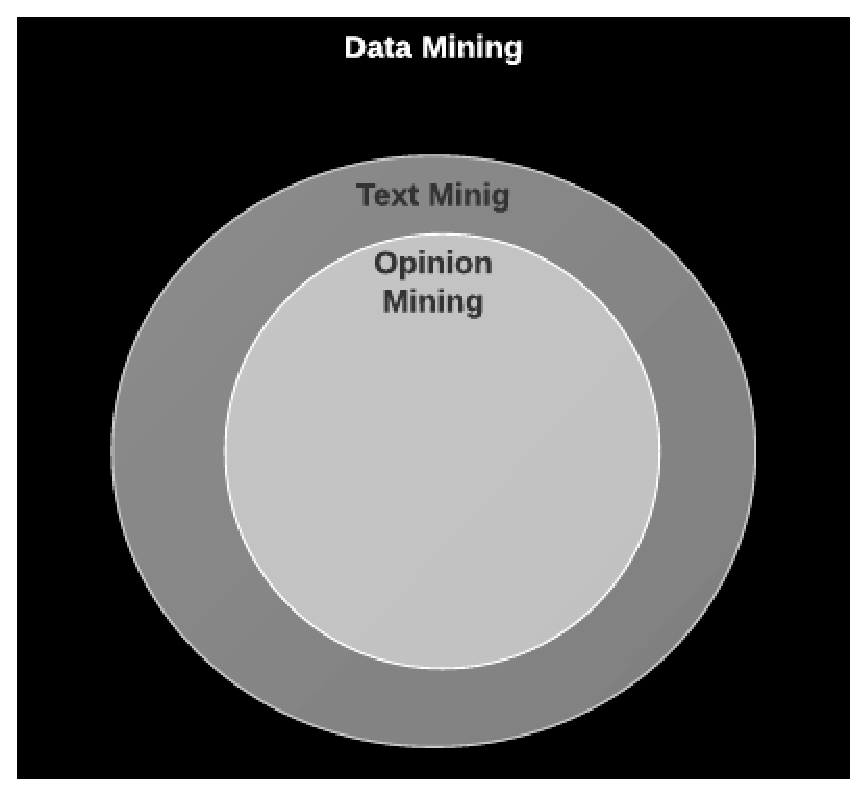
\epsfig{file=figuras/venn.eps, width=5cm}
	\caption{Diagrama de Venn - Mineração de Dados}
	\label{uni}
\end{figure} 

\section{API}\label{sec:api}
* O que é
* APIs mais utilizadas no mundo (case do twitter)
* Papel de uma API para integração de serviços (achar referência foda)

\section{Processamento de linguagem natural}\label{sec:nlp}
* Linguagem natural (foto da matéria de autômato do Aquino?)
* Processamento de linguagem natural
* Dificuldades dentro da nossa área de estudo

\section{Análise de sentimento}\label{sec:analise_sentimento}
* Definição
* Objetivo
* Premissas
* Exemplos e cases de sucesso


\section{Naive Bayes}\label{sec:naive_bayes}
* O que é o Naive Bayes
* Demonstração matemática do algoritmo
* Uso dele em analise de sentimento/classificação


\emph{Naive Bayes} é um algoritmo probabilístico. Baseado no teorema de bayes. $$ P(A \mid B) = \frac{P(B \mid A) \, P(A)}{P(B)} $$ onde se infere qual é a probabilidade de um evento A dado um evento B. Porém nesse trabalho é utilizado o \emph{Naive Bayes} e sua diferença para o teorema de Bayes é assumir que a posição das palavras que aparecem no texto não importa, daí é acrescentado o \emph{naive}(ingênuo) ao teorema.
\\ Como visto em \cite{lucca2013implementaccao} o algoritmo computa qual a probabilidade de uma frase, denominada de documento pertencer a uma determinada classe(polaridade) \emph{P(c/d)}, a partir da probabilidade a \emph{priori} de \emph{P(c)} do documento pertencer a esta classe e da probabilidades condicionais de cada termo \emph{tk} ocorrer em um documento da mesma classe. O algoritmo tem como objetivo encontrar a melhor classe para um documento maximizando a probabilidade a\emph{posteriori} conforme a equação abaixo, onde $ n_{d} $ é o número de termos no documento \emph{d}. $$ C_{map}= argmax_{c \epsilon C}P(c|d)=argmax_{c \epsilon C}P(c)\prod 1sksn_{d}P(t_{k}/d) $$